

%%
%% This is file `sample-manuscript.tex',
%% generated with the docstrip utility.
%%
%% The original source files were:
%%
%% samples.dtx  (with options: `manuscript')
%% 
%% IMPORTANT NOTICE:
%% 
%% For the copyright see the source file.
%% 
%% Any modified versions of this file must be renamed
%% with new filenames distinct from sample-manuscript.tex.
%% 
%% For distribution of the original source see the terms
%% for copying and modification in the file samples.dtx.
%% 
%% This generated file may be distributed as long as the
%% original source files, as listed above, are part of the
%% same distribution. (The sources need not necessarily be
%% in the same archive or directory.)
%%
%% The first command in your LaTeX source must be the \documentclass command.

\documentclass[manuscript,screen,review]{acmart}

\graphicspath{{./}}

\usepackage[main = greek, english]{babel} % For Greek language
\newcommand{\img}[1]
{
    \begin{center}
        \fcolorbox{black}{white}{\includegraphics[height=20em]{#1}}
    \end{center}

}
\usepackage{hyperref}
\usepackage{listings}
\usepackage{graphicx}
\usepackage{float}

% Helper Macros

\newcommand{\en}[1]{\foreignlanguage{english}{#1}}
\newcommand{\src}[1]{{\tt\en{#1}}}

%%
%% End of file `acmart.

\newcommand{\question}[1] % This is what you will use to create a new question
{
\par\noindent % Creates a new unindented paragraph
\phantomsection % Needed for hyperref compatibility with the \addcontensline command
\todo[inline, color=YellowOrange]{\textbf{#1}} % Uses the todonotes package to create a fancy box to put the question
\vspace{1em} % White space after the question before the start of the answer
}


%%
%% \BibTeX command to typeset BibTeX logo in the docs
\AtBeginDocument{%
  \providecommand\BibTeX{{%
    \normalfont B\kern-0.5em{\scshape i\kern-0.25em b}\kern-0.8em\TeX}}}

%% Rights management information.  This information is sent to you
%% when you complete the rights form.  These commands have SAMPLE
%% values in them; it is your responsibility as an author to replace
%% the commands and values with those provided to you when you
%% complete the rights form.
% \setcopyright{}
% \copyrightyear{2023}
% \acmYear{}
% \acmDOI{}

%%
%% Submission ID.
%% Use this when submitting an article to a sponsored event. You'll
%% receive a unique submission ID from the organizers
%% of the event, and this ID should be used as the parameter to this command.
%%\acmSubmissionID{123-A56-BU3}

%%
%% The majority of ACM publications use numbered citations and
%% references.  The command \citestyle{authoryear} switches to the
%% "author year" style.
%%
%% If you are preparing content for an event
%% sponsored by ACM SIGGRAPH, you must use the "author year" style of
%% citations and references.
%% Uncommenting
%% the next command will enable that style.
%%\citestyle{acmauthoryear}

%%
%% end of the preamble, start of the body of the document source.
\begin{document}

%%
%% The "title" command has an optional parameter,
%% allowing the author to define a "short title" to be used in page headers.
\title{Εφαρμογή Διαχείρισης Σταθμών Επαναφόρτισης Ηλεκτρικών Αυτοκινήτων  \\ Εργασία στο μάθημα Βάσεις Δεδομένων - Ακαδημαϊκό Έτος: 2022-23}

%%
%% The "author" command and its associated commands are used to define
%% the authors and their affiliations.
%% Of note is the shared affiliation of the first two authors, and the
%% "authornote" and "authornotemark" commands
%% used to denote shared contribution to the research.



%%
%% By default, the full list of authors will be used in the page
%% headers. Often, this list is too long, and will overlap
%% other information printed in the page headers. This command allows
%% the author to define a more concise list
%% of authors' names for this purpose.

\author{Νικόλαος-Αλκίνοος Αλυσσανδράκης (1072752), Νικόλαος Φιλιππάτος (1072754)}

\authornote{Η εργασία είναι προϊόν ισάξιας συνεισφοράς των δύο συγγραφέων.}
% \email{}
\affiliation{%
  \institution{Tμήμα Ηλεκτρολόγων Μηχανικών και Τεχνολογίας Υπολογιστών}
 % \streetaddress{}
  %\city{ }
 % \state{}
  %\country{}
  %\postcode{}
}


%%
%% The abstract is a short summary of the work to be presented in the
%% article.
\begin{abstract}
\newline
 \en{Command Line Interface } εφαρμογη 
 Η βαση δεδομενων υποστηριζει 
 Διαχειριση χρηστων , αυτοκινητων και σταθμων 

 \end{abstract}

%%
%% The code below is generated by the tool at http://dl.acm.org/ccs.cfm.
%% Please copy and paste the code instead of the example below.
%%


%%
%% Keywords. The author(s) should pick words that accurately describe
%% the work being presented. Separate the keywords with commas.
% \keywords{βάσεις δεδομένων, σχεδιασμός μιας βάσης, διάγραμμα οντοτήτων-συσχετίσεων, σχεσιακό σχήμα, επικοινωνία με την βάση, \en{SQL}}

%%
%% This command processes the author and affiliation and title
%% information and builds the first part of the formatted document.
\maketitle

\newpage

\section{Περιγραφή Προβλήματος}

\subsection{Ένα υποθετικό σενάριο}


Έστω ότι μια εταιρία θέλει να δημιουργήσει στην Ελλάδα ένα μεγάλο δίκτυο σταθμών φόρτισης
ηλεκτρικών αυτοκινήτων. Το δίκτυο αυτό θα αποτελείται από πολλούς σταθμούς, ο καθένας
με αρκετούς φορτιστές και μάλιστα κάθε φορτιστής μπορεί να είναι πολλών ειδών \en{ (AC/DC,}
βύσμα σύνδεσης). Ανά πάσα στιγμή η εταιρεία θέλει να ξέρει την κατάσταση του δικτύου, αν
όλοι οι φορτιστές είναι λειτουργικοί και αν δεν είναι ποια βλάβη αντιμετωπίζουν, πόσοι
φορτιστές είναι κατειλημμένοι και άλλα πολλά στατιστικά σχετικά με το δίκτυο. Παράλληλα
όμως η εταιρία θέλει να διαχειρίζεται και τους πελάτες που χρησιμοποιούν το δίκτυο (άρα
και τα αυτοκίνητά τους), για να ξέρει πόση ενέργεια έχει καταναλώσει ο καθένας, πότε και
με ποιο τρόπο, ώστε εν τέλει να ξέρει πως να τους χρεώσει. Τέλος, η εταιρία επιθυμεί να
δώσει τη δυνατότητα στους πελάτες να δεσμεύουν έναν φορτιστή της επιλογής τους για κάποιο
χρονικό διάστημα.

Για να γίνουν όλα αυτά απαιτείται ένα σύστημα διαχείρισης αυτών των δεδομένων με τρόπο
οργανωμένο και ικανό να αναδείξει τις σχέσεις ανάμεσα σε αυτά, με άλλα λόγια χρειάζεται
μια σχεσιακή βάση δεδομένων.

\subsection{Μικρόκοσμος}

Η σχεδίαση μιας βάσης δεδομένων ξεκινάει από τον ορισμό του μικρόκοσμου, δηλαδή των
οντοτήτων που είναι όντως χρήσιμα και είναι αναγκαίο να συμπεριληφθούν στη βάση, καθώς
και τις σχέσεις μεταξύ τους.

Στην προκειμένη περίπτωση ο μικρόκοσμος θα αποτελείται από τα εξής στοιχεία, με τα εξής
χαρακτηριστικά:

\begin{enumerate}
    \item Οι σταθμοί φόρτισης
    \begin{itemize}
        \item Τοποθεσία
        \item Αριθμός φορτιστών
    \end{itemize}
    \item Οι φορτιστές που βρίσκονται στους σταθμούς
    \begin{itemize}
        \item Τοποθεσία
        \item Κατηγορία φορτιστή (\en{AC/DC})
        \item Τύπος σύνδεσης
    \end{itemize}
    \item Τα σφάλματα που μπορεί να αντιμετωπίζουν οι φορτιστές
    \begin{itemize}
        \item Kωδικός σφάλματος
        \item Στιγμή εμφάνισης
        \item Στιγμή επίλυσης
    \end{itemize}
    \item Οι πελάτες του συστήματος
    \begin{itemize}
        \item Ονοματεπώνυμο
        \item Πρόγραμμα συνδρομής
    \end{itemize}
    \item Τα αμάξια των πελατών
    \begin{itemize}
        \item Αριθμός κυκλοφορίας
        \item Ιδιοκτήτης
        \item Χωρητικότητα μπαταρίας
    \end{itemize}
    \item Τα προγράμματα συνδρομής
    \begin{itemize}
        \item Όνομα προγράμματος
        \item Τιμή παγίου
        \item Τιμή ανά \en{kWh (AC/DC)}
    \end{itemize}
\end{enumerate}

Υπάρχουν επίσης και οι εξής σχέσεις:

\begin{enumerate}
    \item Ένας σταθμός περιλαμβάνει πολλούς φορτιστές
    \item Ένας φορτιστής φορτίζει αμάξια
    \item Ένας φορτιστής μπορεί να αντιμετωπίζει κάποιο πρόβλημα
    \item Ένα αυτοκίνητο ανήκει σε έναν πελάτη
    \item Ένας πελάτης είναι εγγεγραμμένος σε ένα πρόγραμμα συνδρομής
    \item Ένας πελάτης μπορεί να δεσμεύσει έναν φορτιστή για κάποια χρονική διάρκεια
\end{enumerate}

\noindent
Όλες οι οντότητες της βάσης δεδομένων, καθώς και οι σχέσεις μεταξύ τους φαίνονται
ξεκάθαρα στο Σχήμα \en{erd}


\begin{figure}[H]
    \centering
    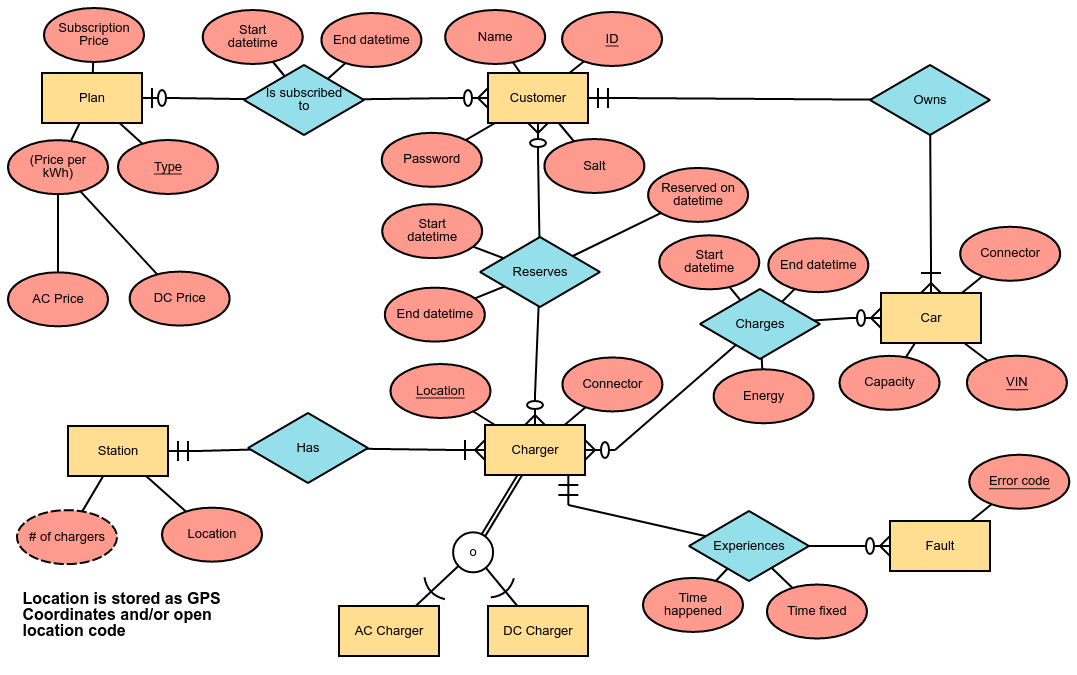
\includegraphics[width=1.1\textwidth]{./Charging Stations.png}
    \caption{Διάγραμμα οντοτήτων συσχετίσεων της βάσης}
\end{figure}


\newpage
\subsection{Σχεσιακό Μοντέλο }

Βασιζόμενοι στο \en{erd} κατασκευάσαμε και το σχεσιακό μοντέλο με την \en{online } εφαρμογη \en{dbdesigner.net}
Ακολουθήσαμε την θεωρία των βάσεων όπως έχουμε πει στο μάθημα και στο εργαστήριο.
Οι σχέσεις μεταξύ των οντοτήτων μεταφράστηκαν στο σχεσιακό ξεχωριστούς πίνακες . 
Φροντίσαμε 


\begin{figure}[H]
    \centering
    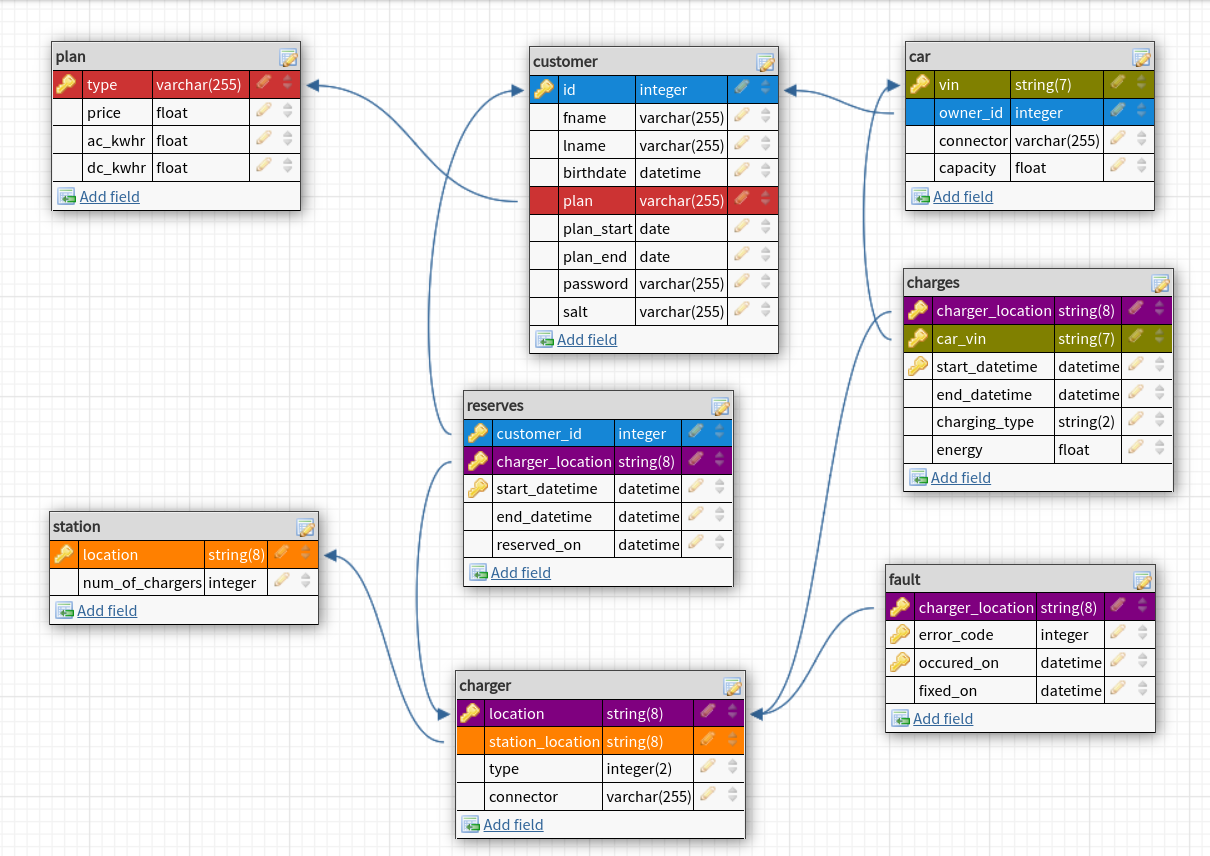
\includegraphics[width=1.1\textwidth]{./DBDesigner.png}
    \caption{Σχεσιακό Μοντέλο της βάσης}
\end{figure}

\newpage


\section{Μεθοδολογία-Προσέγγιση}
\label{method}

Αρχικά πραγματοποιήσαμε έρευνα σχετικά με ήδη υπάρχοντα συστήματα διαχείρισης σταθμών
επαναφόρτισης ηλεκτρικών αυτοκινήτων, μέσω τις οποίας καταγράψαμε οι βασικές απαιτήσεις
που πρέπει να έχει ένα τέτοιο σύστημα. Ύστερα σκεφτήκαμε τις οντότητες και τις σχέσεις
ανάμεσα σε αυτές, τις οποίες χρειάζεται το σύστημα προκειμένου να καλύψει όλες τις
απαιτήσεις που είχαμε θέσει. Από αυτές τις σκέψεις προέκυψε το διάγραμμα σχέσεων
οντοτήτων (Σχήμα \ref{erd}). Στη συνέχεια χρησιμοποιήσαμε αυτό το διάγραμμα προκειμένου
να σχεδιάσουμε τη δομή της βάσης δεδομένων χρησιμοποιώντας το εργαλείο DB Designer.

Μετά από αυτό το βήμα αρχίσαμε να υλοποιούμε το πρόγραμμα με παράλληλο τρόπο. Ο ένας
ασχολήθηκε με τη διεπαφή του χρήστη με το πρόγραμμα \en{(command line interface)}, ενώ
ο άλλος ασχολήθηκε με τη δημιουργία της βάσης και η εισαγωγή των δεδομένων, καθώς και
την επικοινωνία του προγράμματος με τη βάση δεδομένων.\newline\newline 

\section{Χωρισμός Τμημάτων}
\label{division}

\subsection{Αλκίνοος Αλυσσανδράκης}
\label{alkinoos}

\begin{itemize}
    \item Εισαγωγή δεδομένων στη βάση (όπως αυτό αναλύθηκε στο τμήμα \ref{data})
    \item Επικοινωνία του προγράμματος με τη βάση δεδομένων για το κομμάτι που αφορά την
        εισαγωγή και εξαγωγή δεδομένων και πληροφοριών από το σύστημα (λειτουργίες
        στατιστικών, δέσμευσης φορτιστών, καταγραφής φορτίσεων, καταγραφή σφαλμάτων)
\end{itemize}

\subsection{Νικόλας Φιλιππάτος}
\label{nikolas}

\begin{itemize}
    \item Διεπαφή του χρήστη με το πρόγραμμα
    \item Επικοινωνία του προγράμματος με τη βάση δεδομένων για το κομμάτι που αφορά τους
        χρήστες και την εξουσιοδότηση τους (προσθήκη και εύρεση χρηστών, επαλλήθευση
        κωδικόυ πρόσβασης, προσθήκη και εύρεση αυτοκινήτων)
\end{itemize}

\newpage 

\section{Προγραμμα}

\begin{itemize}
    \item \en{Python}
    \item \en{python module sqlite}
    \item \en{python module bcrypt} 
\end{itemize}

Για την ανάπτυξη της εφαρμογής μας , χρησιμοποιήσαμε την γλώσσα \en{python } . 
Την χωρίσαμε σε 6 αρχεία. 

\begin{itemize}
    \item  \en{main.py} : Κύριο πρόγραμμα
    \item  \en{cli.py}  : Διεπαφή με τον χρήστη
    \item  \en{creating\_database.py} : Δημιουργία βάσης δεδομένων
    \item  \en{filling\_database.py} : Δημιουργία δεδομένων και εισαγωγής στην βαση
    \item  \en{user.py} : Επικοινωνια με την βάση για ενέργειες σχετικά με τον χρήστη
    \item  \en{database\_class.py } : Επικοινωνία με την βάση
\end{itemize}


\subsection{\en{main.py}}


 Συνδέει κάποια αρχεία μεταξύ τους . Δέχεται ορίσματα στο τρέξιμο του ( \en{-f/--file } για να προσδιοριστεί το αρχείο βάσης με το οποίο θέλουμε να τρέξει η εφαρμογή ) . 
 Εάν δεν δοθεί κάποιο αρχείο θα τρέξει με την προκαθορισμένο αρχείο \en{data.db} . 
 Εδώ θα μπορούσε να πάρει ένα ακόμα όρισμα και να τρέχει το \en{gui} . 


\subsection{\en{cli.py}}

 Προβάλλει πληροφορίες για την εφαρμογή στον χρήστη και διαχειρίζεται τις αιτήσεις του . Τρέχει ένα \en{menu} που προβάλλει τις επιλογές που μπορεί να κάνει ο χρήστης και διαχειρίζεται την επιλογή του. Οι συναρτήσεις ειναι γραμμένες με τρόπο που υποστηρίζονται και απο μια γραφική διεπαφή  που κληρονομεί την κλαση της \en{App}.
 


 \subsection{\en{creating\_database.py}}

 Με την χρηση της βιβλιοθήκης \en{sqlite3}, συνδέεται με την βάση δεδομένων και εκτελεί τα \en{queries} που δημιουργούν τους πίνακες δεδομένων, με το καταλληλο \en{format} και τους αντίστοιχους περιορισμούς. 

 \subsection{\en{filling\_database.py}}

 Η επικοινωνία με την βάση γινεται πάλι με την χρήση της βιβλιοθήκης sqlite3 . 
Γεμίζουμε τους πίνακες \en{charger,customer,plan,station} με χρήσιμα δεδομένα. Συγκεκριμένα τα \en{plan,station} έχουν καποιες \en{standard} τιμές που παίρνουν . Οι  \en{charger,station } για την τοποθεσία χρησιμοποιούν κωδικούς \en{open location codes }  

\subsection{\en{user.py}}

 Διαχειρίζεται την είσοδο του χρήστη στην εφαρμογή και αντίστοιχα την εγγραφή του . Επικοινωνεί με την βάση για να πάρει τις κατάλληλες πληροφοριες . Το \en{ID } καθε χρήστη ειναι μοναδικό και το \en{Primary key }. Οι κωδικοί του χρήστη αποθηκεύονται στην βάση κρυπτογραφημένοι με την βιβλιοθήκη \en{bcrypt} και την συναρτηση της \en{hashpw()} , μαζί με μια φράση \en{salt} που φροντίζει την ασφάλεια της κρυπτογράφησης. 

 


\subsection{\en{database\_class.py}}

 Τελος το αρχειο \en{database\_class.py} διαχειρίζεται τα ερωτήματα που κάνει το πρόγραμμα μας στην βάση . Κάθε συναρτηση αφορά και διαφορετική ερώτηση , επιστρέφοντας λίστες με αποτελέσματα των σειρών των απαντήσεων.

 

\newpage
\section{Δεδομένα}
\label{data}

Η εισαγωγή των δεδομένων στη βάση έγινε σε δύο στάδια. Αρχικά με το πρόγραμμα
\en{filling\_database.py} δημιουργήθηκαν τα δεδομένα για τους πίνακες \en{customer, plan, chargers}
και \en{station}. Το πρόγραμμα αυτό χρησιμοποιεί μια λίστα με αγγλικά ονόματα για να
δημιουργήσει τα ονόματα των χρηστών και προκαθορισμένες λίστες τιμών για τα υπόλοιπα
πεδία, με τρόπο τέτοιο ώστε να υπάρχει ποικιλία στα παραγόμενα δεδομένα. Στη συνέχεια
χρησιμοποιήθηκε το \en{online} εργαλείο \en{Mockaroο} για να δημιουργηθούν τα δεδομένα των πινάκων
\en{charges, reserves, faults}. Το εργαλείο αυτό επιτρέπει, μέσα από τον ορισμό του σχήματος
του πίνακα και ορισμένων παραμέτρων για κάθε στήλη, την αυτόματη δημιουργία αρκετών
δεδομένων. Στο εργαλείο \en{Mockaroo} έγινε είσοδος των δεδομένων που είχαν παραχθεί από το
πρόγραμμα \en{python} και χρησιμοποιήθηκαν προκειμένου να παραχθούν τα υπόλοιπα. Όλα τα
δεδομένα από το \en{Mockaroo} παράχθηκαν σε μορφή αρχείων \en{CSV} (βρίσκονται στον φάκελο \en{sqldata}) και εισήχθησαν στη βάση μέσω
του εργαλείου \en{sqlitebrowser}



\section{Χρήση Προγράμματος}

 Πρώτα απόλα πηγαίνουμε στον φάκελο που περιέχει τα προγράμματα . 

  Τρέχουμε την εντολή :
  \selectlanguage{english}
    \begin{lstlisting}
        pip3 install -r requirements.txt
    \end{lstlisting}
    \selectlanguage{greek}
Που εγκαθιστά τις βιβλιοθήκες που θα χρησιμοποιήσουμε . \newline\newline

 Για να τρέξουμε την εφαρμογή τρεχουμε το πρόγραμμα \en{main.py} στον ιδιο φακελο που εχουμε την βαση μας. Εαν δεν εχουμε εύκαιρη την βάση , δημιουργείται αυτόματα, αλλα πρεπει να εισαγουμε και τα \en{cvs} δεδομενα απο τον φακελο  \en{sqldata}

 Εάν γνωρίζουμε το \en{id} και \en{password} καποιου χρηστη προχωραμε στην συνδεση του . Αλλιως κανουμε εγγραφη , προσφεροντας τα απαραιτητα στοιχεια. 
 
 Ο κωδικος \en{id}:0 ειναι πιασμενος για τον λογαριασμο \en{admin}  με κωδικο \en{admin}\newline

 Για τους υπολοιπους χρηστες στον πινακα \en{customer} o κωδικος του καθενος ειναι το \en{firstname}

 Για αυτους που εχουν ξεχάσει τον λογαριασμό τους υπαρχει η δυνατοτητα υπενθυμισης του \en{id}.

 Τελος υπαρχει και η επιλογη να δει καποιος ενδεικτικα στατιστικα στοιχεια για τους σταθμους. 

 Μετα την συνδεση του , ο χρηστης μπορει να δει πληροφοριες για τον λογαριασμο του και τα αμαξια που ειναι στο ονομα του , να δει στατιστικα στοιχεια που τον αφορουν , να προσθεσει αμαξι , να αλλαξει κωδικο και να κανει δεσμευση μιας συγκεκριμενης ωρας ενος σταθμου για να μπορει να παει να φορτισει το αυτοκινητο του (δεν ειναι πληρως λειτουργικο ) .\newline\newline 

 Ο χρηστης \en{admin} εχει την δυνατοτητα να βλεπει στατιστικα στοιχεια που αφορουν τους σταθμους και δεν ειναι προσβασιμα στο απλο κοινο και να επιδιορθωνει τα σφαλματα . 
 
\newpage
\section{Αξιολόγηση}

Η εφαρμογη μας μπορει να δημιουργησει νεους χρηστες και να συνδεθει σε υπαρχοντες. Δειχνει γενικα στατιστικα στοιχεια για τους σταθμους φορτισης. Τα δεδομενα που εχουμε βαλει στην βαση επιστρεφουν μια προσομοιωση κανονικης λειτουργιας.

Δυστυχως δεν καταφεραμε να υλοποιησουμε την διαδικασια δεσμευσης φορτιστων απο τους χρηστες, παρολο που προσφερει μια τετοια δυνατοτητα η βαση μας .
Οι κωδικοι των χρηστων αποθηκευονται κρυπτογραφημενοι με την βιβλιοθηκη \en{bcrypt} μαζι με το \en{salt} που βοηθαει την κρυπτογραφηση και αποκρυπτογραφηση . 

Για την τοποθεσια των σταθμων προχωρησαμε στην χρηση των open \en{location codes ()} το οποιο μπορει να χρησιμοποιηθει και \en{offline} , και με την χρηση \en{gps} στα αμαξια θα μπορουσε να υπολογισει και την βελτιστη διαδρομη για να παει σε εναν ελευθερο φορτιστη πριν ξεμεινει απο ενεργεια . 



\section{Χρονοδιάγραμμα}

Την πρωτη εβδομαδα του Νοεμβριου, λαμβανοντας την εκφωνηση της εργασιας συζητησαμε και καταγραψαμε τον μικροκοσμο του προβληματος μας δημιουργώντας και το διάγραμμα οντοτήτων-συσχετίσεων . Μέχρι το τέλος του Νοεμβρίου είχε γραφτεί και το σχεσιακό μοντέλο  . 
Οι πρώτες 3 εβδομάδες του Δεκεμβρίου αφορούσαν την δημιουρία της διεπαφής με τον χρήστη . Η τελική απόφαση ήταν να γίνει το πρόγραμμα διεπαφή γραμμής εντολών (\en{command line interface}) . Οι συναρτήσεις έχουν κατασκευαστεί με τέτοιο τρόπο ώστε μια γραφική διεπαφή να κληρονομεί τις συναρτήσεις που ελέγχουν τα δεδομένα και να γιίνει αντικατάσταση των συναρτήσεων που δέχονται δεδομένα από τον χρήστη και προβάλλουν τα αποτελέσματα. 
Μέσα στις διακοπές των χριστουγέννων υλοποιήθηκαν οι ερωτήσεις που πραγματοποιεί η εφαρμογή στην βάση μας .



\section{Βιβλιογραφία}
\begin{itemize}
    

      \item \en{https://www.sqlite.org/index.html} : \en{Documentation}
      \item \en{https://erdmaker.com/editor} 
      \item \en{https://www.dbdesigner.net/} : Σχεσιολογικο Μοντελο 
      \item \en{https://mockaroo.com/} : Δεδομενα για βαση
      \item \en{https://github.com/smashew/NameDatabases.git}: Ονοματα για πελατες
      \item \en{https://github.com/google/open-location-code} : Τεχνολογια για τοποθεσια 
      \item \en{https://www.tutorialspoint.com/sqlite/sqlite\_python.htm}
      
      
\end{itemize}


\newpage
\section{Παράρτημα}

\subsection{Σύνδεσμοι}
\en{Github Repository link}: \en{\url{https://github.com/nikolasfil/Database---Charging-Stations}}

\subsection{Eφαρμογή Εν Δράση }

\begin{figure}[H]
    \centering
    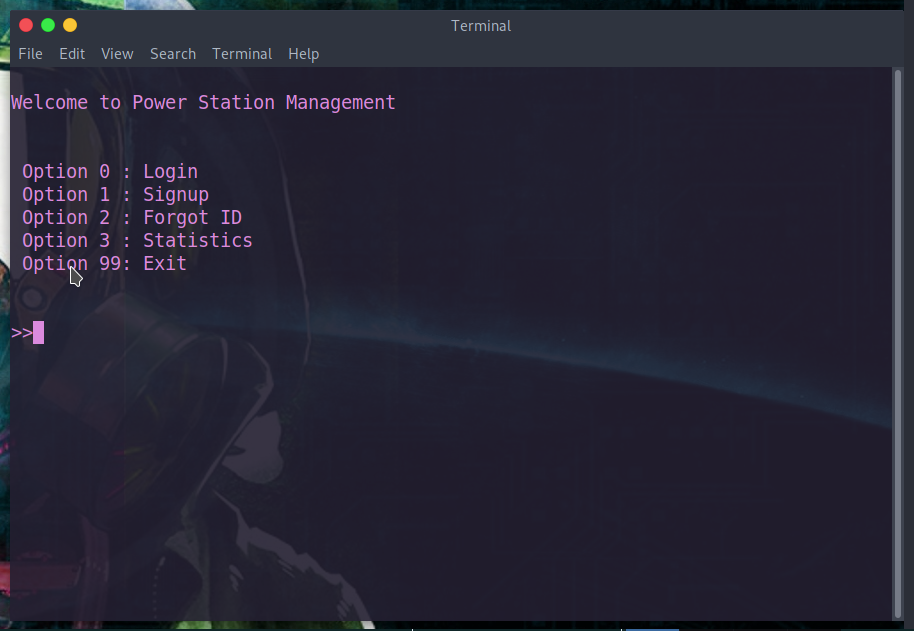
\includegraphics[width=.7\textwidth]{./db_main_page.png}
    \caption{\en{main page}}
\end{figure}

\begin{figure}[H]
    \centering
    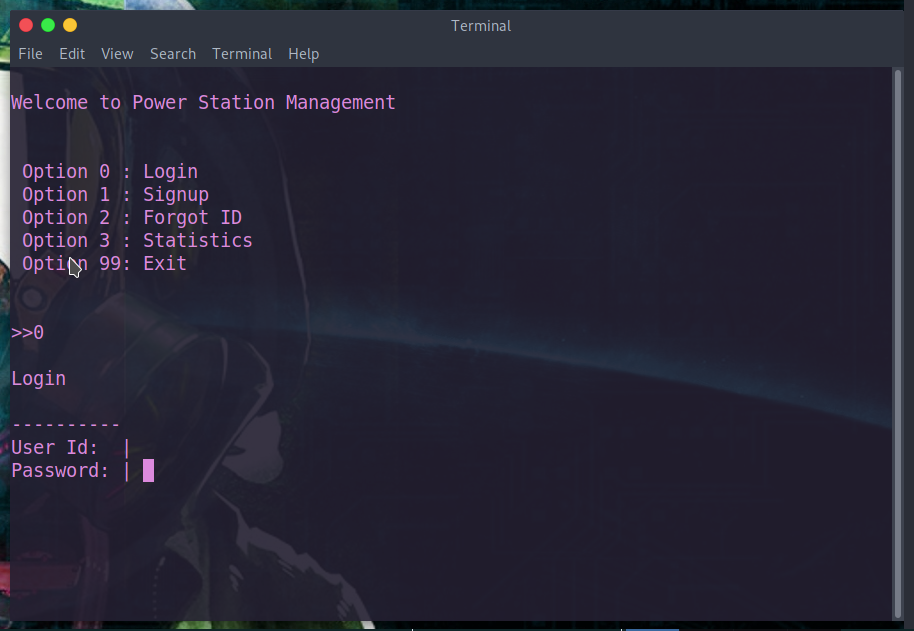
\includegraphics[width=.7\textwidth]{./db_login_option.png}
    \caption{\en{login}}
\end{figure}

\begin{figure}[H]
    \centering
    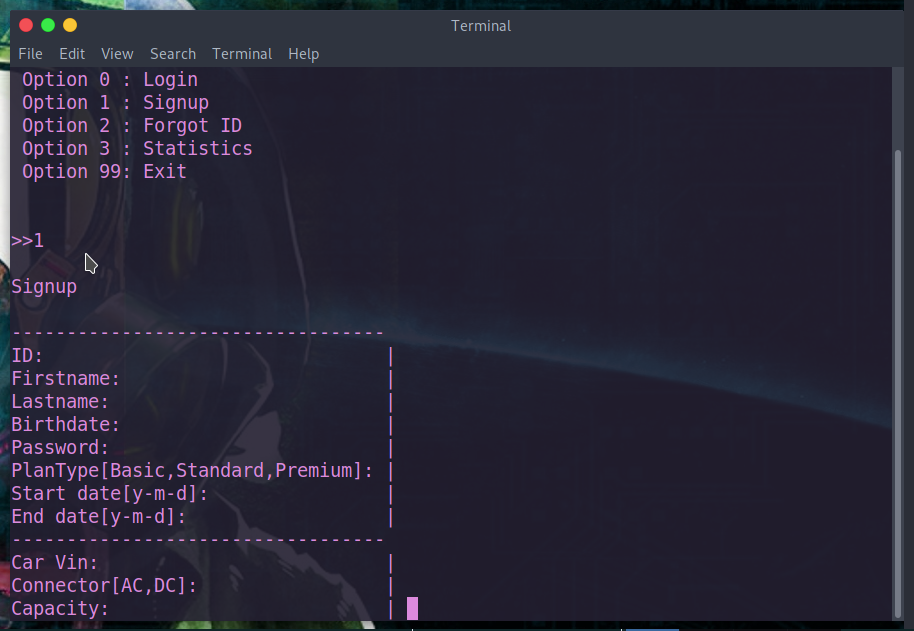
\includegraphics[width=.7\textwidth]{./db_signup.png}
    \caption{\en{sign up }}
\end{figure}


\begin{figure}[H]
    \centering
    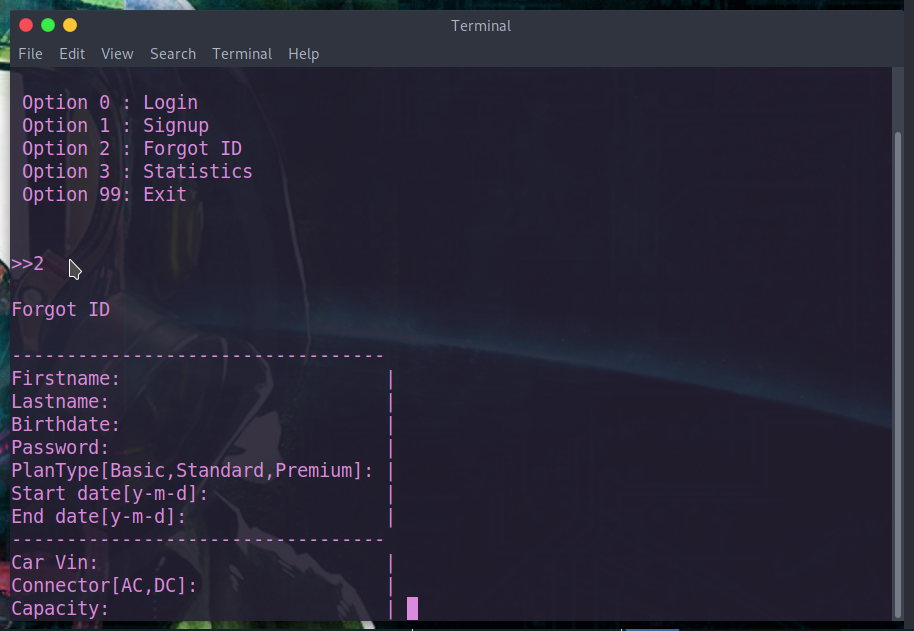
\includegraphics[width=.7\textwidth]{./db_forgot_id.png}
    \caption{\en{forgot id}}
\end{figure}


\begin{figure}[H]
    \centering
    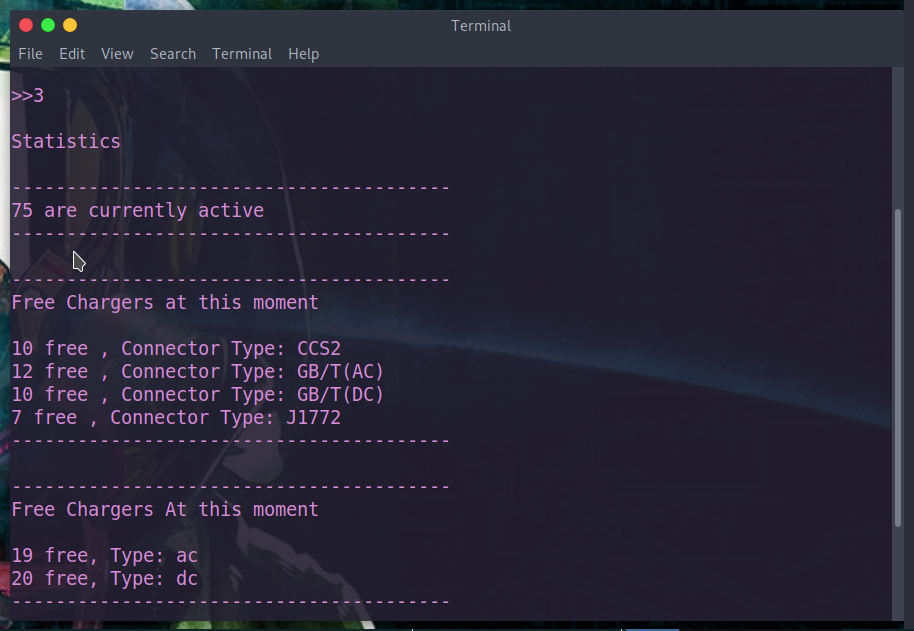
\includegraphics[width=.7\textwidth]{./db_statistics.png}
    \caption{\en{statistics}}
\end{figure}

\newpage


\begin{figure}[H]
    \centering
    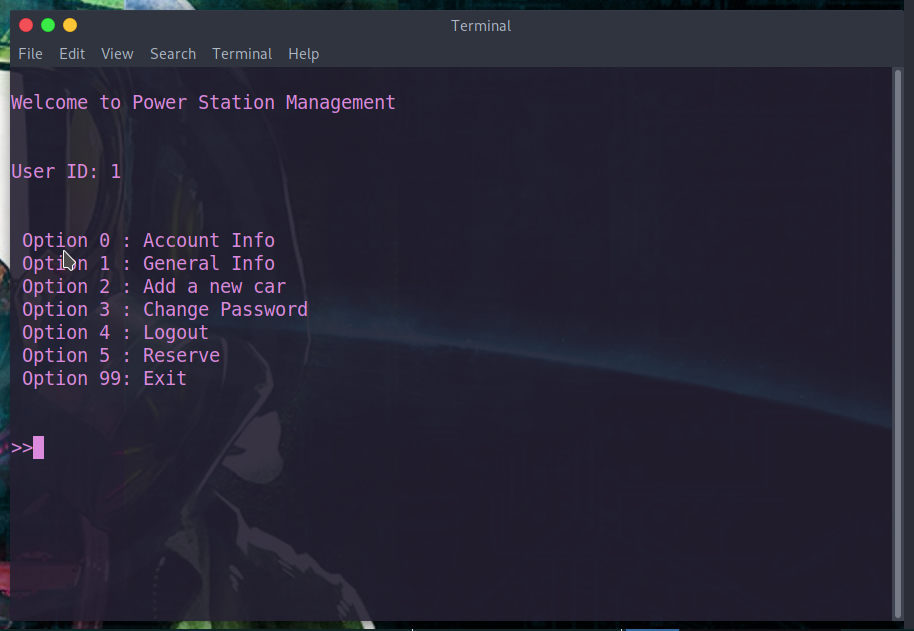
\includegraphics[width=.7\textwidth]{./db_aaron_main.png}
    \caption{\en{Aaron Main}}
\end{figure}

\begin{figure}[H]
    \centering
    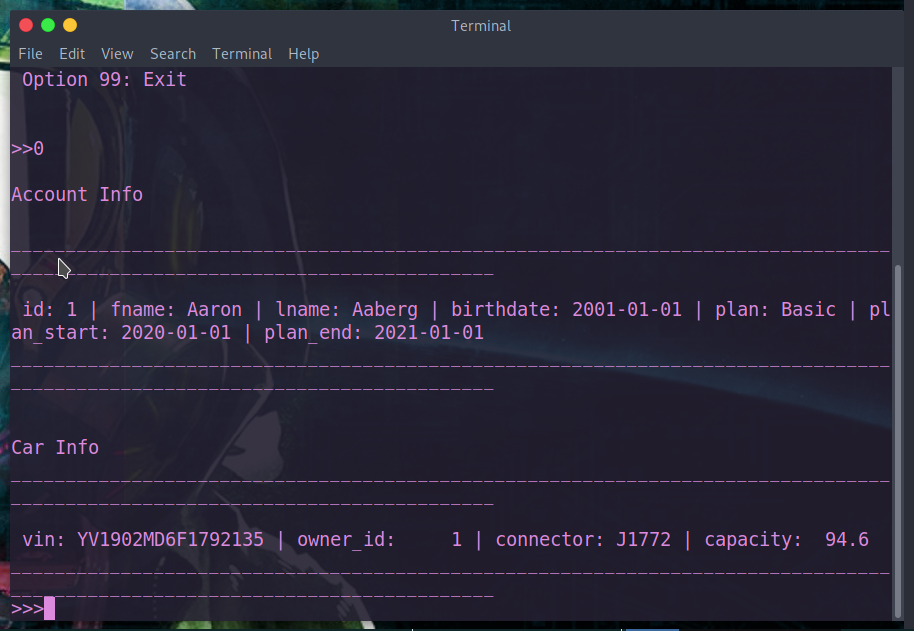
\includegraphics[width=.7\textwidth]{./db_aaron_info.png}
    \caption{\en{Aaron Account Info }}
\end{figure}


\begin{figure}[H]
    \centering
    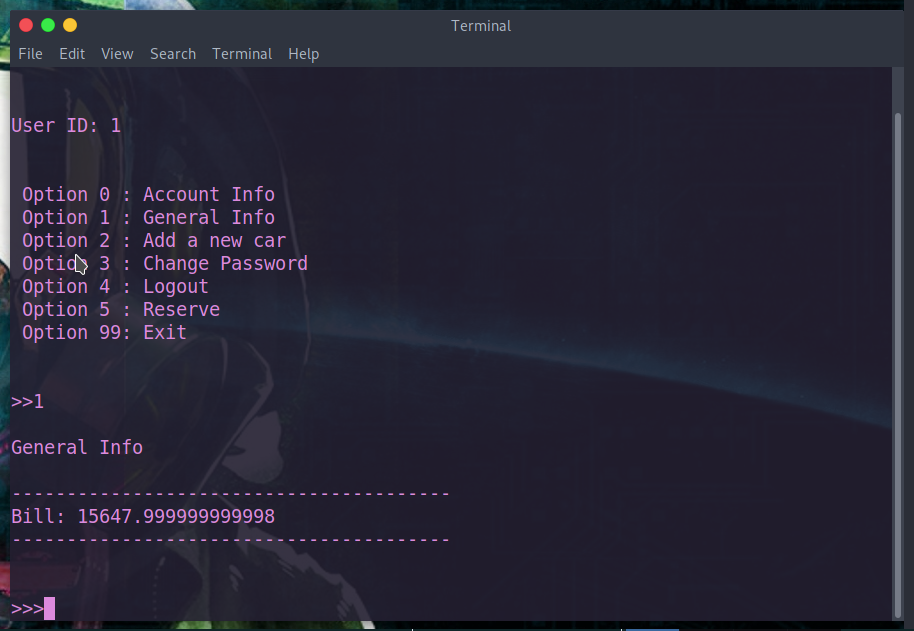
\includegraphics[width=.7\textwidth]{./db_aaron_general.png}
    \caption{\en{Aaron General Info }}
\end{figure}

\begin{figure}[H]
    \centering
    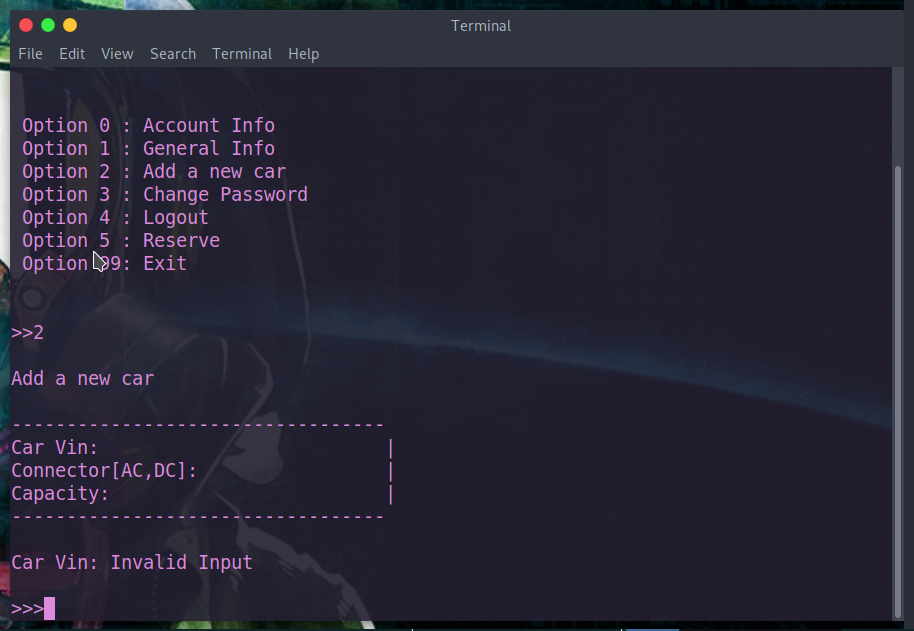
\includegraphics[width=.7\textwidth]{./db_aaron_add_car.png}
    \caption{\en{Aaron New Car }}
\end{figure}

\begin{figure}[H]
    \centering
    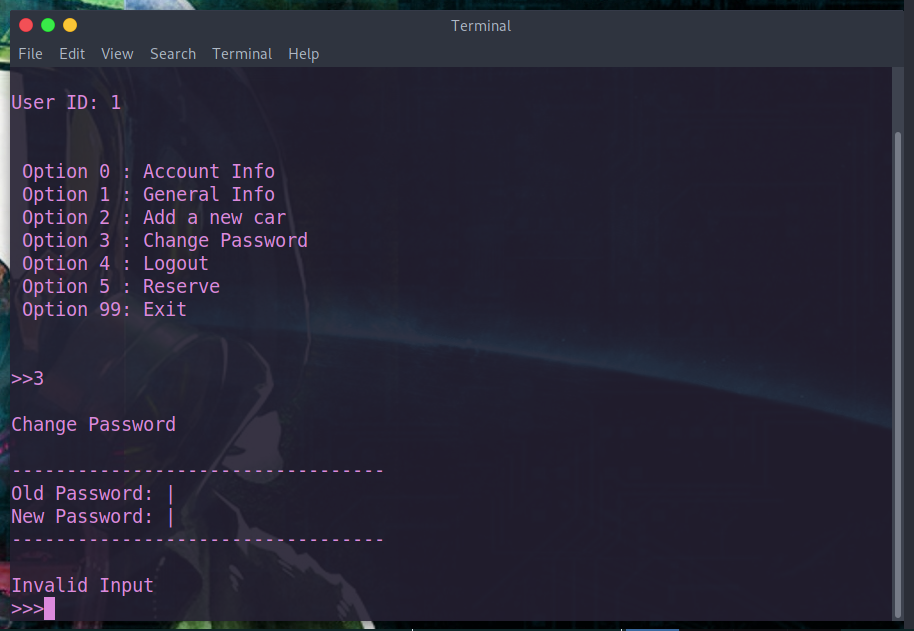
\includegraphics[width=.7\textwidth]{./db_aaron_change.png}
    \caption{\en{Aaron Change Password }}
\end{figure}

\begin{figure}[H]
    \centering
    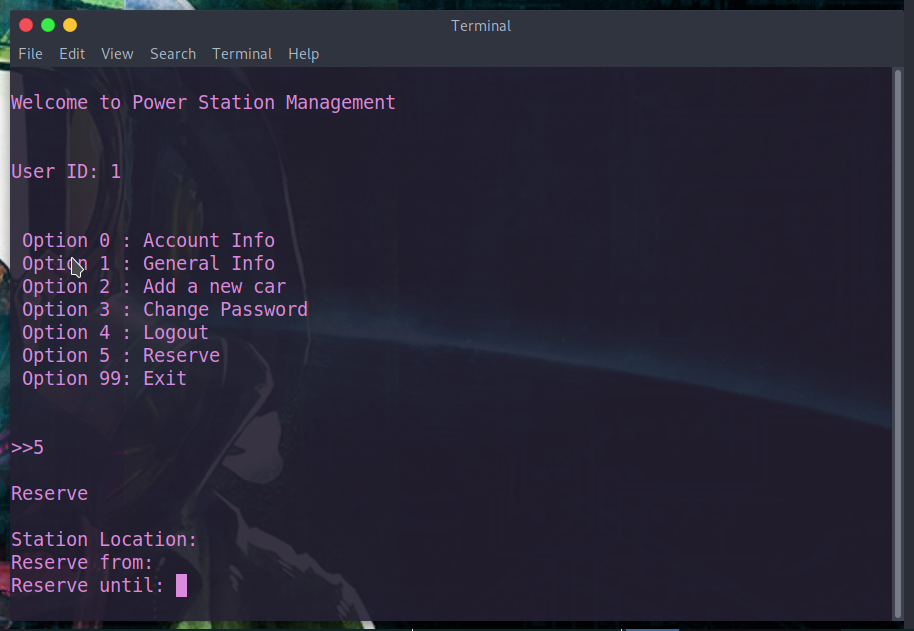
\includegraphics[width=.7\textwidth]{./db_aaron_reserve.png}
    \caption{\en{Aaron Reserve }}
\end{figure}

\newpage

\begin{figure}[H]
    \centering
    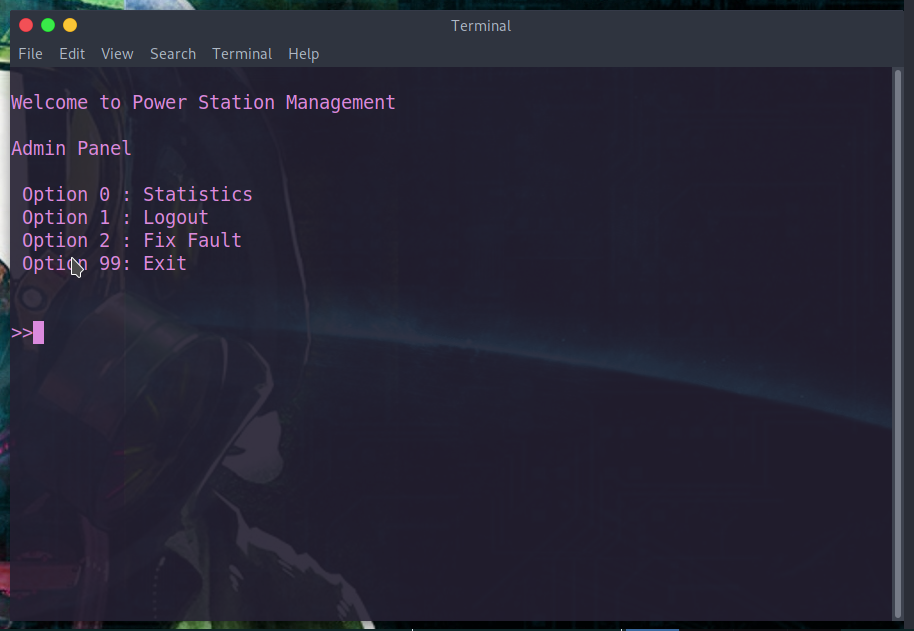
\includegraphics[width=.7\textwidth]{./db_admin_main.png}
    \caption{\en{Admin Main page }}
\end{figure}


\begin{figure}[H]
    \centering
    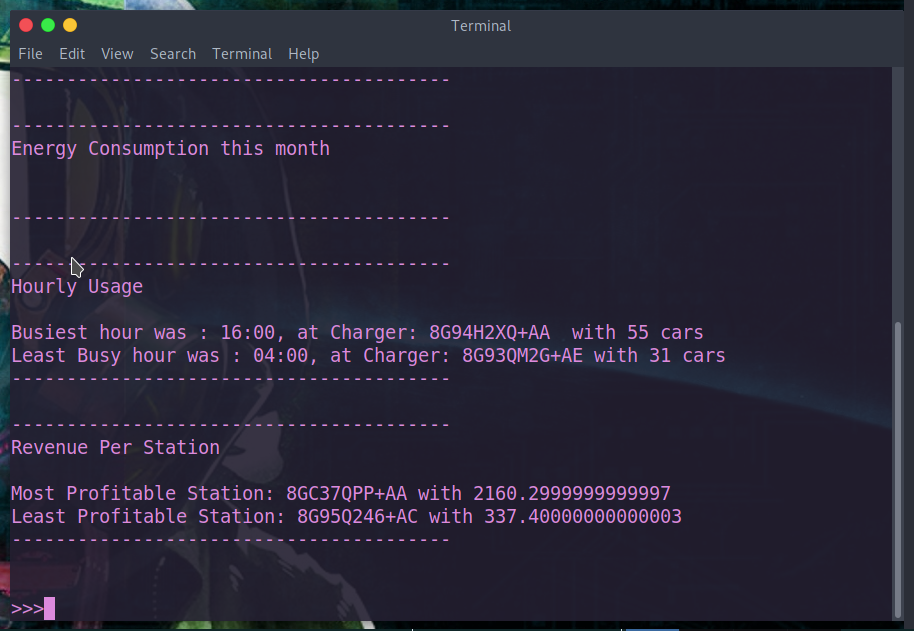
\includegraphics[width=.7\textwidth]{./db_admin_statistics.png}
    \caption{\en{Admin statistics }}
\end{figure}


\begin{figure}[H]
    \centering
    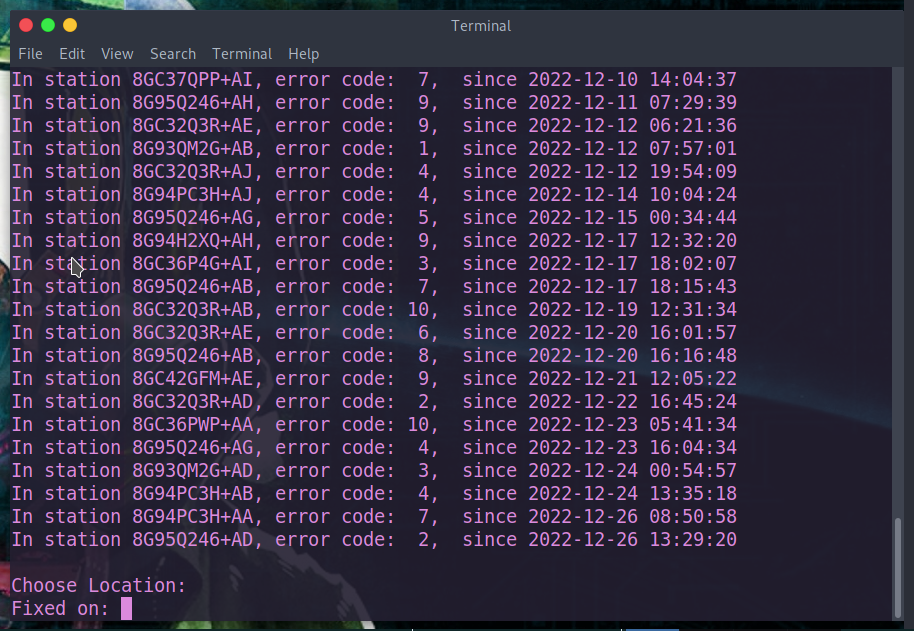
\includegraphics[width=.7\textwidth]{./db_admin_fix.png}
    \caption{\en{Admin Fix Faults }}
\end{figure}

\end{document}
\endinput
%%
%% End of file `sample-manuscript.tex'.
